% Se conserva únicamente el apéndice B solicitado.
\setcounter{chapter}{1}
\chapter{Logs y datos complementarios}

\section{Evidencia de pruebas con fork bomb}

La primera prueba se presenta directamente en el capítulo de resultados. Este
anexo conserva la salida original de la segunda corrida como evidencia
complementaria de la carga crítica.

Las capturas se presentan en el orden entregado: inicio de la corrida crítica,
resumen de resultados y estado observado con 616 procesos.

\begin{figure}[H]
  \centering
  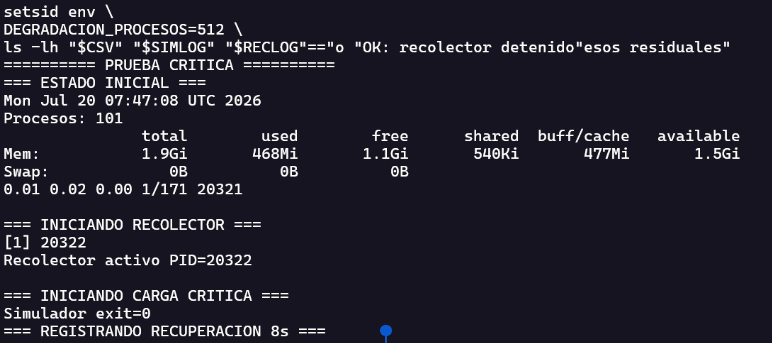
\includegraphics[width=0.94\textwidth]{figuras/anexos/fork_prueba_2_inicio.png}
  \caption{Prueba 2: estado inicial, inicio del recolector y ejecución de la carga crítica.}
  \label{fig:fork-p2-inicio}
\end{figure}

\begin{figure}[H]
  \centering
  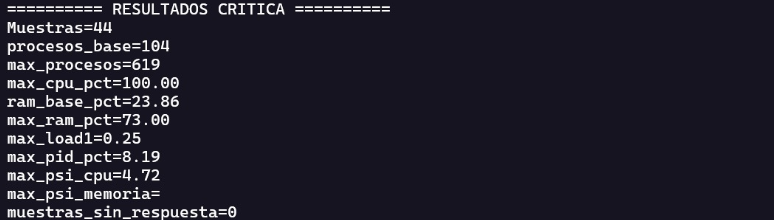
\includegraphics[width=0.94\textwidth]{figuras/anexos/fork_prueba_2_resultados.png}
  \caption{Prueba 2: resumen de mediciones de la carga crítica.}
  \label{fig:fork-p2-resultados}
\end{figure}

\begin{figure}[H]
  \centering
  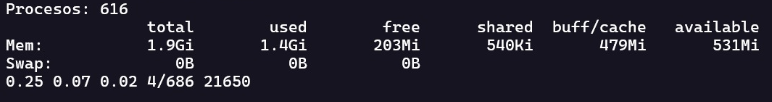
\includegraphics[width=0.94\textwidth]{figuras/anexos/fork_prueba_2_estado.png}
  \caption{Prueba 2: estado observado con 616 procesos y uso de memoria de la máquina virtual.}
  \label{fig:fork-p2-estado}
\end{figure}
